\documentclass{article}

\usepackage{graphicx}
\usepackage{hyperref}
\usepackage[a4paper, margin=1.25in]{geometry}
\usepackage{breakcites}
\usepackage{subcaption}
\usepackage{float}
\usepackage{textcomp}
\usepackage{amsmath}
\usepackage{textgreek}
\usepackage{authblk}
\usepackage{rotating}
\usepackage{booktabs}
\usepackage{longtable}
\usepackage{pdflscape}
\usepackage{subcaption}
\usepackage{lineno}
\usepackage[
  style=numeric,
  citestyle=numeric-comp,
  backend=biber,
  doi=true,
  natbib=true,
  sorting=none
]{biblatex}

\pagestyle{fancy}
\fancyhf{}
\lfoot{Supplemental Materials for \textit{Fine-scale Twitter Big Data Reveals Neighborhood Inequalities in Mental Health Effects of High Temperatures}}
\rfoot{\thepage}

\renewcommand{\footrulewidth}{0.4pt}
\renewcommand{\headrulewidth}{0pt}


\addbibresource{TextDataClimateShocks.bib}

\begin{document}
\begin{center}
\section*{Supplemental Materials for \textit{Fine-scale Twitter Big Data Reveals Neighborhood Inequalities in Mental Health Effects of High Temperatures}}
\end{center}

%Supplement will have:

%Equations used for RH and WBGT

\section{Alternative Parameterizations}

\section{Effects of Precipitation and Sunshine}

\section{Alternative Sentiment Algorithm}

\setcounter{table}{0}
\setcounter{figure}{0}
\setcounter{section}{0}
\renewcommand{\thetable}{S\arabic{table}}
\renewcommand{\thefigure}{S\arabic{figure}}
\renewcommand{\thesection}{S\arabic{section}}

\printbibliography

\end{document}

\section*{Supplemental Info}
\setcounter{table}{0}
\setcounter{figure}{0}
\setcounter{section}{0}
\renewcommand{\thetable}{S\arabic{table}}
\renewcommand{\thefigure}{S\arabic{figure}}
\renewcommand{\thesection}{S\arabic{section}}

\begin{figure}[H]
  \centering
  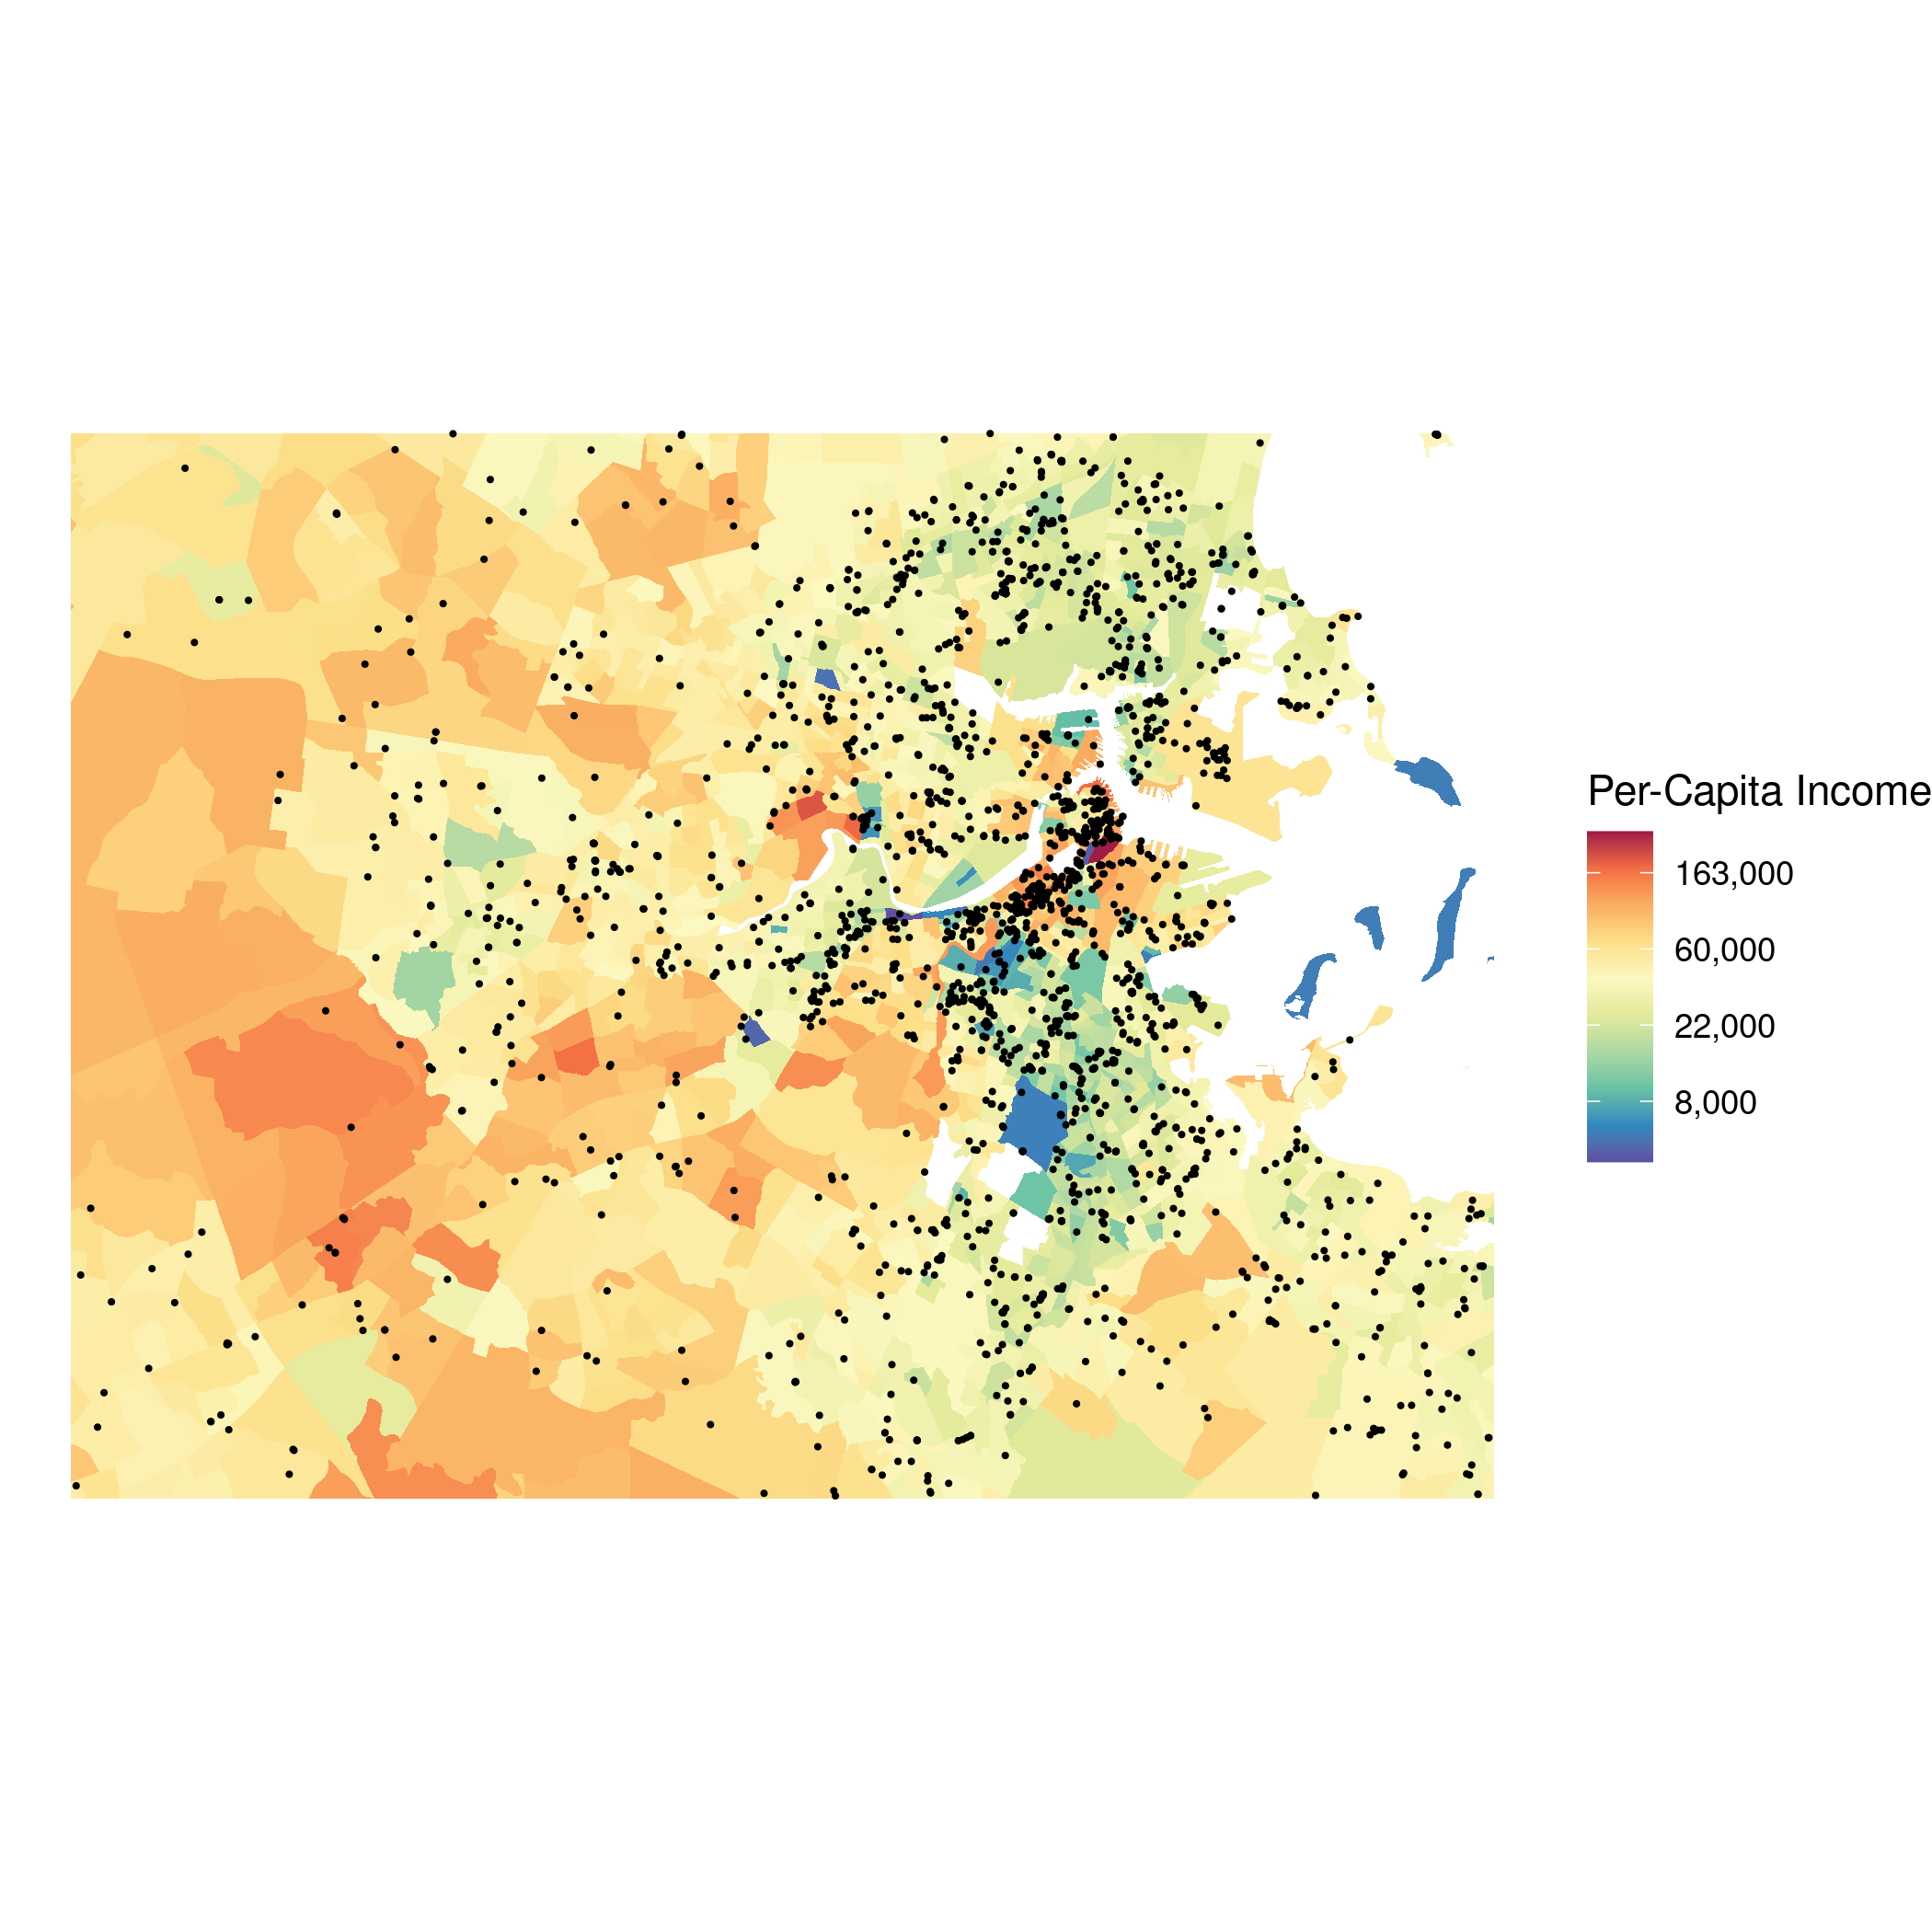
\includegraphics[width=\linewidth]{../res/Boston_Map.png}
  \caption{Here is a map of all tweets in boston, overlaid with income by census block}
  \label{fig:timeseries}
\end{figure}

\begin{figure}[H]
  \centering
  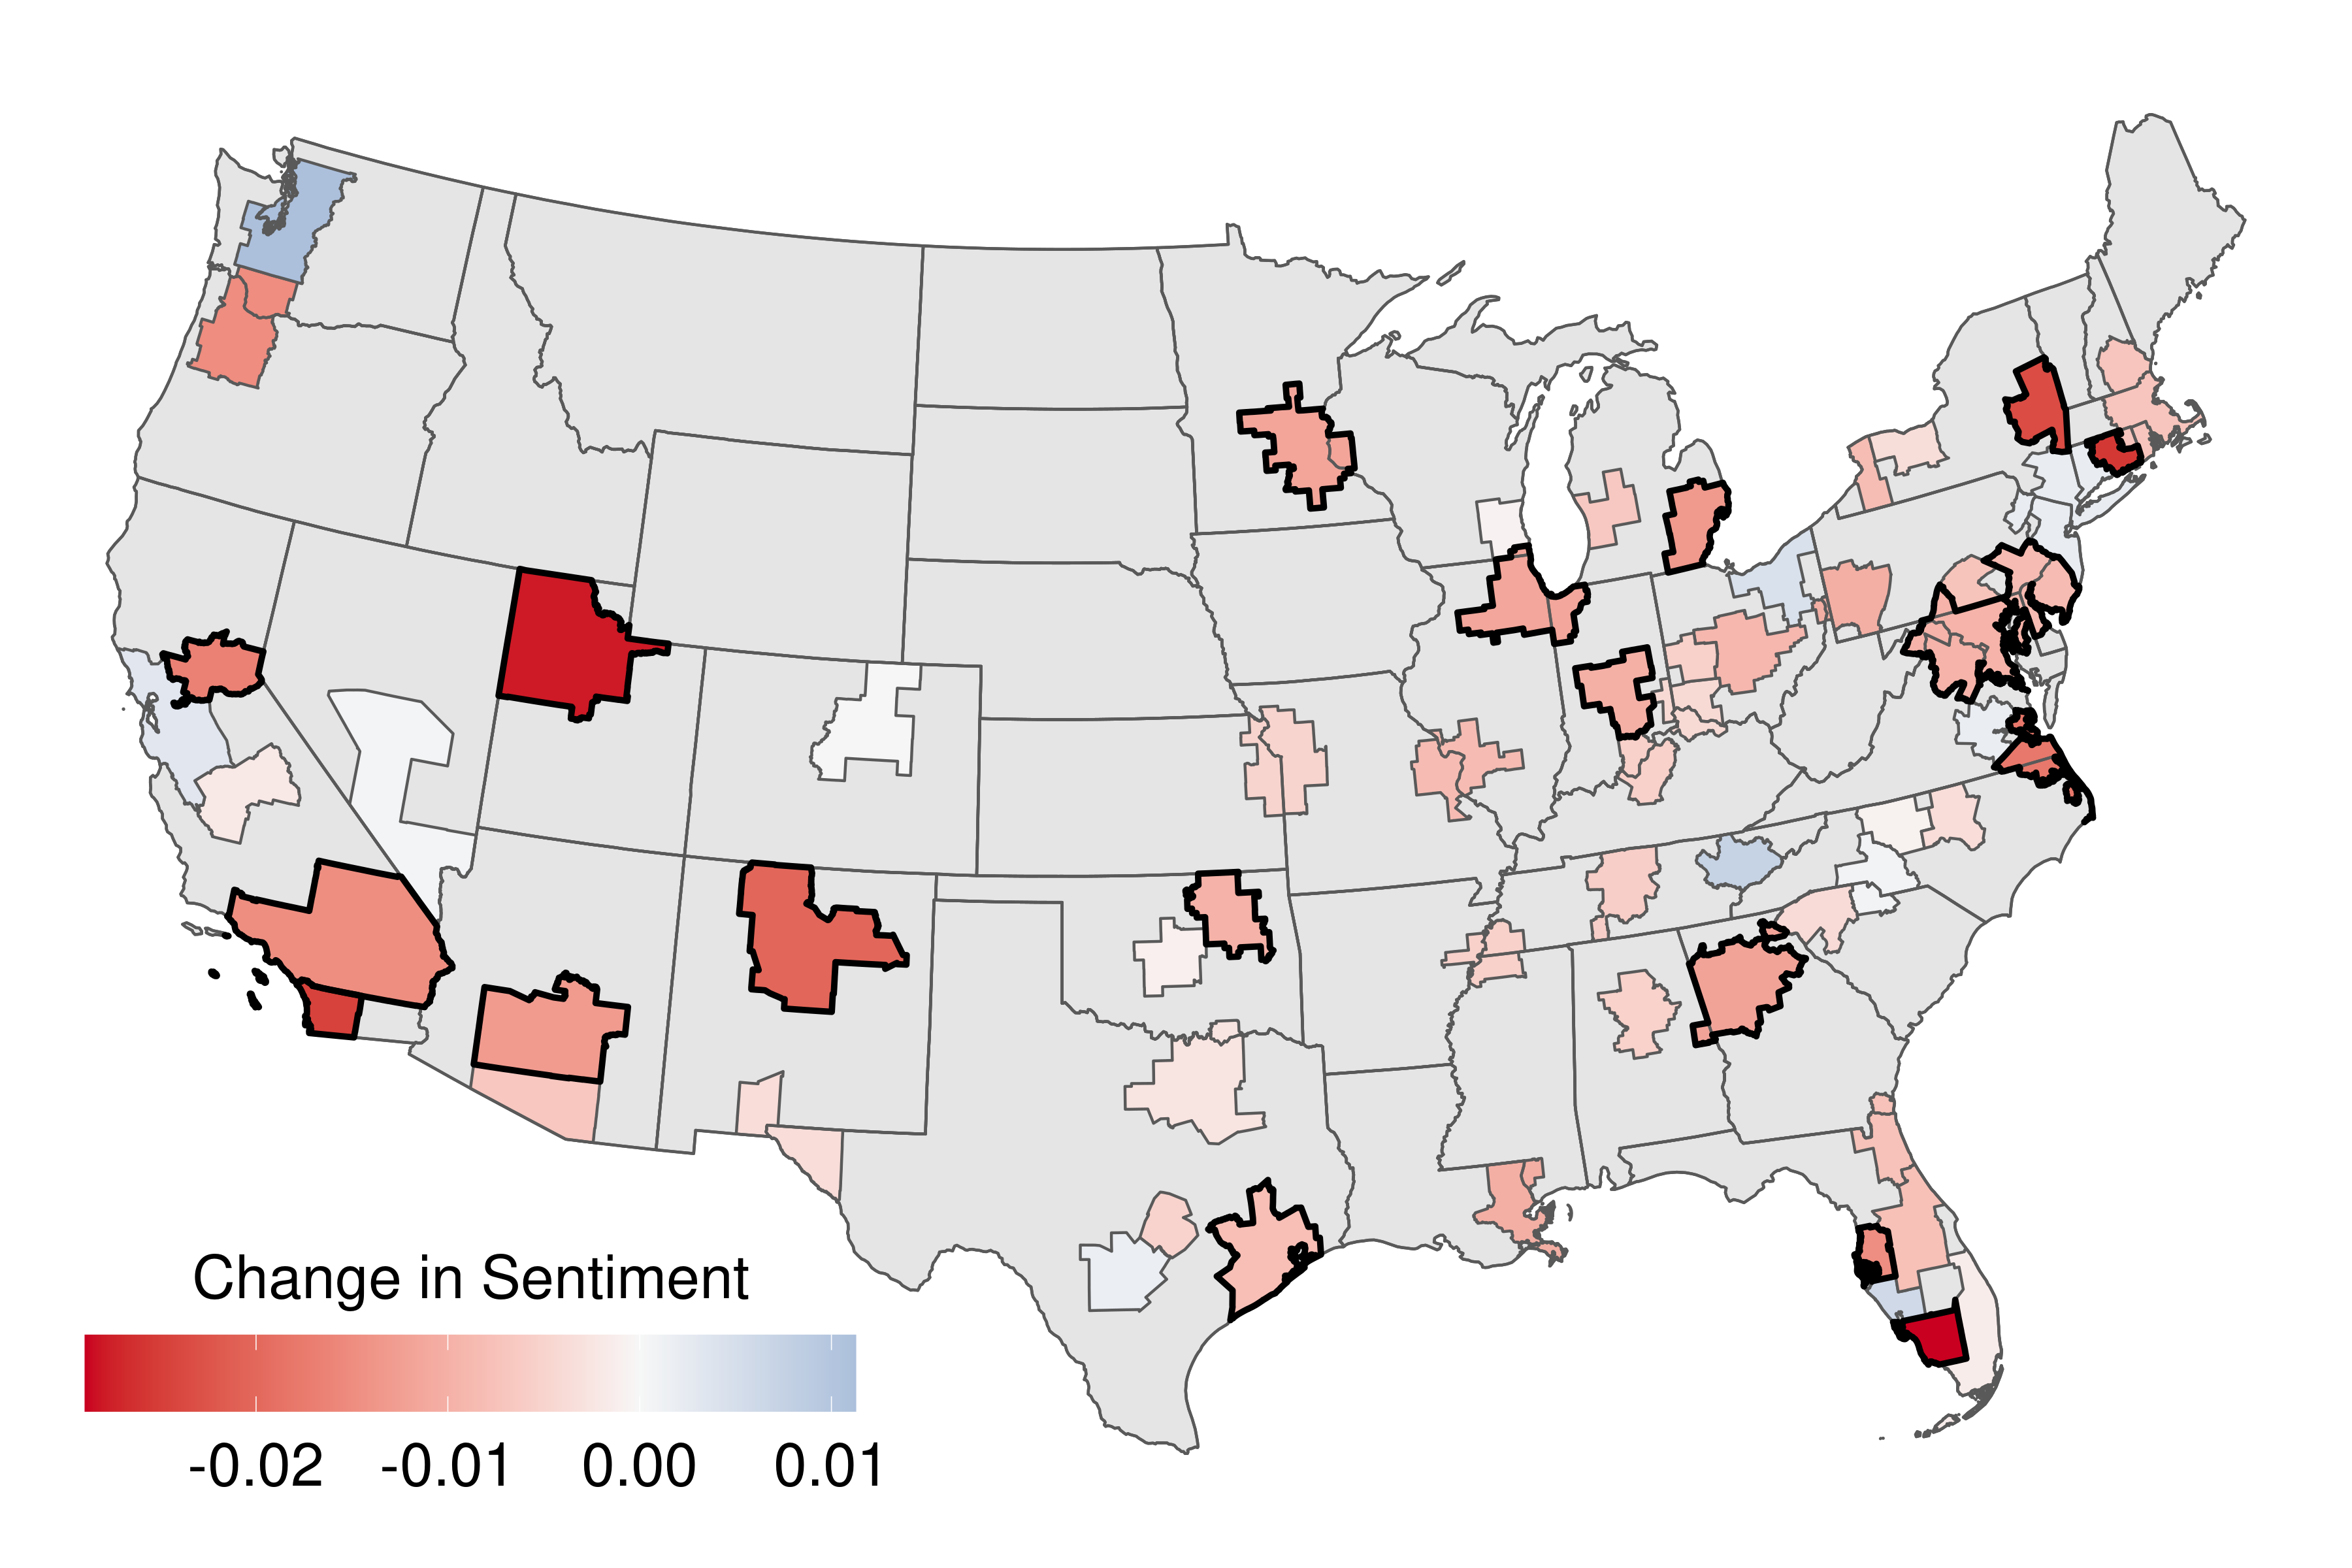
\includegraphics[width=\linewidth]{../res/map_wbgt.png}
  \caption{Here is a map of all tweets in boston, overlaid with income by census block}
  \label{fig:timeseries}
\end{figure}


\end{document}
